\documentclass[a4paper,12pt]{ThesisStyle}
\usepackage[utf8]{inputenc}
\usepackage{thesis-style}
\usepackage{parskip}
\usepackage{beramono}
\usepackage[section]{placeins}

\begin{document}

\frontmatter

\pagenumbering{gobble}

\thispagestyle{empty}
\begin{table}[htb]
  \centering
  \begin{Large}
    \resizebox{\textwidth}{!}{\begin{tabular}{| l |}
        \hline
        \\
        \includegraphics[scale=0.9]{/assets/logos/EPS.png}                                 \\[0.7cm]
        \centerline{Projecte fi de grau}                                                   \\[1cm]
        \hline
        \\
        \textbf{Estudi}: Grau en Enginyeria Informàtica                                    \\[0.7cm]
        \hline
        \\
        \textbf{Títol}: Eina de suport per a l’elaboració dels horaris dels graus de l’EPS \\[0.7cm]
        \hline
        \\
        \textbf{Document}: Memòria                                                         \\[0.7cm]
        \hline
        \\
        \textbf{Alumne}: Adrià Ribas Chico                                                 \\[0.7cm]
        \hline
        \\
        \textbf{Tutor 1}: Dra. Marta Fort Masdevall                                        \\
        \textbf{Departament}: Informàtica, matemàtica aplicada i estadística               \\
        \textbf{Àrea}: Llenguatges i sistemes informàtics                                  \\[0.7cm]
        \hline
        \\
        \textbf{Tutor 2}: Dr. Antonio Rodríguez Benítez                                    \\
        \textbf{Departament}: Informàtica, matemàtica aplicada i estadística               \\
        \textbf{Àrea}: Llenguatges i sistemes informàtics                                  \\[0.7cm]
        \hline
        \\
        \textbf{Convocatòria (mes/any)}: Juny de 2022                                      \\[0.7cm]
        \hline
      \end{tabular}}
  \end{Large}
\end{table}

\newpage

\begin{titlepage}

  % Upper part of the page
  \includegraphics[scale=0.9]{/assets/logos/EPS.png} \\[1cm]
  \begin{center}
    \textsc{\Large Projecte Fi de Grau} \\[1cm]

    % Title
    \begin{spacing}{2}
      \HRule \\
      \textbf{\Huge Eina de suport per a l’elaboració dels horaris dels graus de l’EPS} \\
      \HRule \\[0.5cm]
    \end{spacing}

    % Author and supervisor and other data
    {
    \large
    \emph{Autor:} \\
    Adrià \textsc{Ribas Chico} \\[1cm]
    Juny de 2022 \\[1cm]
    Grau en Enginyeria Informàtica \\[1cm]
    \emph{Tutors:} \\
    Dra. Marta \textsc{Fort Masdevall} \\
    Dr. Antonio \textsc{Rodríguez Benítez} \\
    }

  \end{center}
\end{titlepage}

\titlepage

\dominitoc

\pagenumbering{roman}

\chapter*{Resum}
\label{cap:resum}

El resum del projecte va aquí \ldots

\chapter*{Agraïments}
\label{cap:agraiments}

Agraïments \ldots


\tableofcontents

%\listoffigures

%\listoftables

\mainmatter

\chapter{Introducció}
\label{cap:intro}

\section{Antecedents}
\label{sec:antecedents}

En aquesta secció, es resumiran els antecedents que han donat peu al plantejament d'aquest projecte.

La idea del projecte neix de determinades necessitats que cert personal de l'Escola Politècnica Superior de la Universitat de Girona fa temps que té. Més concretament, es tracta d'una necessitat del personal encarregat de gestionar tot el que fa referència a la confecció i manteniment dels horaris del centre: horaris dels graus, dels professors, ocupació d'aules i espais, etc.

Actualment, per dur a terme l'elaboració dels horaris, aquestes persones utilitzen mètodes i eines incòmodes i poc àgils, a part de no estar automatitzades ni específicament dissenyades per abordar aquest tipus de tasques. Tampoc existeix cap plataforma que unifiqui les fases d'aquest procés de gestió ni que n'estableixi una manera de fer comuna.

Ara per ara, per exemple, no tenen manera de detectar incompatibilitats horàries ni solapaments \textit{a priori} de manera automàtica. Degut a això, en moltes ocasions s'han de repetir certes fases del procés fins que el resultat és vàlid i la gent implicada hi està d'acord.

Al capítol~\ref{cap:marcdetreball} es descriurà amb més profunditat com funcionen avui en dia aquests processos d'elaboració i gestió d'horaris de l'escola.

\section{Propòsit}
\label{sec:proposit}

En aquesta secció, s'exposarà el propòsit general del projecte, tenint en compte els antecedents vists a la secció~\ref{sec:antecedents}.

En definitiva, la gestió dels horaris de l'EPS suposa una inversió de temps massa elevada per a la gent que se n'ocupa. És per això que la Dra. Marta Fort Masdevall, coordinadora d'estudi del Grau en Enginyeria Informàtica de la universitat, proposa un projecte de fi de grau que té la finalitat de trobar una solució al problema.

El propòsit és desenvolupar una eina de suport informàtic que permeti a l'usuari elaborar horaris de forma àgil, eficient i segura. L'eina també hauria de ser capaç de comprovar automàticament la disponibilitat de les aules, les incompatibilitats horàries dels professors i la concordança entre les assignatures i el nombre de grups previstos. A més a més, hauria d'oferir diverses vistes per tal que l'usuari pugui visualitzar la informació, com ara:
\begin{itemize}
  \item Els horaris d'un grau per curs i quadrimestre.
  \item Els horaris d'un professor per quadrimestre.
  \item L'ocupació d'un espai per quadrimestre.
\end{itemize}

També es planteja la possibilitat de disposar d'un sistema de control d'usuaris. Cada usuari tindria assignat un conjunt de rols determinat. Els rols representarien els diferents càrrecs del personal de l'EPS en matèria de gestió d'horaris. Així doncs, cada usuari podria executar les accions i consultar la informació que el seu conjunt de rols li permeti. D'aquesta manera, es dividirien les diferents tasques i processos entre rols d'usuari i cadascun dels càrrecs podria realitzar la feina que li correspon. La proposta inicial comprèn els rols d'usuari següents:
\begin{itemize}
  \item \texttt{Administrador}: Introdueix les aules i els grups previstos.
  \item \texttt{Coordinador}: Elabora els horaris.
  \item \texttt{Director de departament}: Dóna d'alta responsables de docència.
  \item \texttt{Responsable de docència}: Dóna d'alta i assigna professors als grups.
  \item \texttt{Professor}: Visualitza el seu horari.
\end{itemize}

A més a més, l'aplicació hauria de ser accessible via web. D'aquesta manera, tots els usuaris podrien utilitzar-la des de qualsevol lloc i dispositiu, sense preocupar-se d'instal·lacions ni actualitzacions.

\section{Motivacions}
\label{sec:motivacions}

En aquesta secció, es parlarà en primera persona sobre quines motivacions personals hi ha darrere del projecte i en justifiquen l'elecció.

Un dels aspectes que més em motiven de la informàtica en general és el fet de poder ajudar la gent a estalviar el seu temps, el qual penso que és de gran valor. En moltes ocasions, una persona, un grup o fins i tot una institució, inverteix una quantitat elevada de temps en realitzar certes accions o activitats, sigui en l'àmbit que sigui. Aquest temps es pot reduir si l'acció o activitat en qüestió té una part suficientment mecànica. Tanmateix, encara que no la tingui, sovint és possible desenvolupar una eina informàtica que n'augmenti l'eficiència o, si més no, dinamitzar-la i fer que resulti més còmoda i pràctica.

D'aquí sorgeix el meu objectiu principal pel que fa a la informàtica, que és precisament aportar el meu gra de sorra a aquesta causa.

Per aquest motiu, m'ha cridat molt l'atenció la proposta d'aquest projecte. És una molt bona oportunitat per contribuir a millorar el procés de gestió i elaboració d'horaris de l'escola, que sol resultar bastant costós en temps per a les persones que hi participen.

D'altra banda, em motiva molt el fet de desenvolupar una aplicació que podrà ser implantada en un entorn real i que podrà beneficiar les persones que la facin servir. No em cridaria tant dur a terme un altre projecte que, un cop finalitzat, fos simplement arxivat, sense utilitat pràctica per a ningú més excepte per a mi, que seria l'únic que me'n beneficiaria, ja que igualment obtindria coneixements i experiència.

Actualment i cada vegada més, m'interessa el desenvolupament d'entorns web. És per això que un factor decisiu a l'hora d'escollir aquesta proposta de PFG ha estat que un dels requisits sigui desenvolupar-lo en format de plataforma web.

\section{Objectius generals}
\label{sec:objectius_generals}

En aquesta secció, s'enumeraran els objectius generals del projecte, que ja s'han deixat entreveure prèviament a la secció~\ref{sec:proposit}. No obstant això, a continuació se'n presenta la llista completa:
\begin{itemize}
  \item Proporcionar una interfície còmoda i intuïtiva per dur a terme les tasques de gestió i elaboració dels horaris de l'EPS.
  \item Emmagatzemar i processar dinàmicament les dades i relacions referents als diversos graus, cursos, quadrimestres, assignatures, grups, espais, professors, etc.
  \item Detectar i evitar automàticament qualsevol tipus d'inconsistència o incompatibilitat horària, per tal d'aportar seguretat al treball.
  \item Possibilitar la pujada d'arxius externs de dades que serveixin per obtenir la informació bàsica necessària per al funcionament de l'aplicació i generar possibles punts de partida per a la planificació dels horaris.
  \item Permetre la visualització de l'ocupació de les aules, dels horaris dels professors i dels horaris dels grups de cada grau, entre d'altres vistes que puguin ser d'utilitat pels usuaris.
  \item Admetre diferents rols d'usuari, als quals s'assigni una sèrie de tasques i un conjunt de permisos concret.
\end{itemize}

Al capítol~\ref{cap:requisits} es desenvoluparan aquests objectius generals i es concretaran els requisits específics de l'aplicatiu.


%%%%%%%%%%%%%%%%%%%%%%%%%%%%%%%%%%%%%%%%%%%%%%%%%%%%%%%%%%%%%%%%%%%%%%%%%%%%%%%%%%%%%%%%%%%%%%%%%%%%%%%%%%%%%%%%%%%%%%%%%%%%%%%%%%%%%%%%%%%%%%%%%%%%%
\section{-------------- EXEMPLES I UTILITATS --------------}
\subsection{Paraules per començar seccions}
\textbf{Idees:}

Abordar, concretar, exposar, parlar, descriure, repassar, mostrar, ensenyar, desenvolupar, tractar, veure, aprofundir, investigar, discutir, indagar, detallar,
enumerar,


\subsection{Altres}

Això és un exemple de citació d'un llibre~\cite{Coleman1974}, un article científic~\cite{Ruiz2008} i una referència a una web~\cite{Halcon}.

Exemple de taula:
\begin{table}[htb]
  \centering
  \begin{tabular}{ | r | c | c | l | }
    \hline
    Any  & Matriculats & Aprovats & Percentatge \\
    \hline
    2019 & 65          & 47       & 72.3\%      \\
    2020 & 69          & 48       & 69.6\%      \\
    2021 & 75          & 58       & 77.3\%      \\
    \hline
  \end{tabular}
  \caption{\label{taula:taulaexemple} Aquí és on s'ha de posar el peu de taula. }
\end{table}

Exemple de figura:
\begin{figure}[htb]
  \centering
  \includegraphics[width=8 cm]{/assets/logos/EPS.png}
  \caption{\label{fig:logo} Logotip de l'Escola Politècnica Superior.}
\end{figure}

Exemple de fòrmula:
\begin{equation}
  H(X) = -\sum_{i=1}^{N}p_s(x_i) \log \left( p_s(x_i) \right).
  \label{equ:entropia}
\end{equation}


També es pot fer referència en el text a les taules (p.ex. veure la Taula~\ref{taula:taulaexemple}), a les figures (p.ex. veure la Figura~\ref{fig:logo}) o a les fòrmules (p.ex. veure Equació~\ref{equ:entropia}).

%%%%%%%%%%%%%%%%%%%%%%%%%%%%%%%%%%%%%%%%%%%%%%%%%%%%%%%%%%%%%%%%%%%%%%%%%%%%%%%%%%%%%%%%%%%%%%%%%%%%%%%%%%%%%%%%%%%%%%%%%%%%%%%%%%%%%%%%%%%%%%%%%


\chapter{Viabilitat}
\label{cap:viabilitat}



\chapter{Metodologia}
\label{cap:metodologia}



\chapter{Marc de treball i conceptes previs}  % Els noms de les seccions són provisionals, per posar-hi algo
\label{cap:marcdetreball}

\section{Conceptes previs}
\label{sec:conceptes_previs}
Explicar setmanes a i b, assignatures compartides, què són els blocs (especials també)..., quantes hores
són un crèdit, ¿explicar funcions de cada rol?...

\section{Funcionament actual}
\label{sec:funcionament_actual}

En aquesta secció, es detallaran quins són i com funcionen els mètodes de gestió i elaboració d'horaris de l'EPS que s'utilitzen actualment. Es veuran quins càrrecs de l'escola hi participen i les seves funcions, així com la manera en què interactuen entre ells i intercanvien la informació corresponent.

Parlar del flux dels processos, etc \ldots

Rectorat reparteix crèdits a les facultats. Cada facultat decideix quants grups grans, petits, etc. de cada grau en funció dels alumnes. Introdueix els excels.
A partir d'aquí, entren els coordinadors, per fer els horaris amb els seus mètodes. Canviar-los el mínim possible respecte l'any passat, per intentar evitar
solapaments. Un cop fets, els coordinadors passen els horaris a direcció. S'entren al sistema i revisen solapaments. Si tot està bé, els responsables de docència,
que assignen professors als grups.

Grups grans i mitjans no hi ha restriccions d'aules. Grups petits sí,

\section{Tecnologies}
\label{sec:tecnologies}

Explicar tecnologies.

\chapter{Requisits del sistema}
\label{cap:requisits}

\section{Consideracions inicials}
\label{sec:consideracions_inicials}

En aquesta secció, es presentaran una sèrie de consideracions inicials amb l'objectiu de clarificar el contingut de les seccions que segueixen.

En primer lloc, és necessari definir el format que adoptarà cadascun dels requisits del sistema:
\\[8pt]
\centerline{\texttt{\textbf{Tipus-Numeració [Prioritat]}}: Descripció}

Més concretament, el tipus de requisit es representarà mitjançant les seves sigles, com ara \texttt{RF} pels funcionals o \texttt{RNF} pels no funcionals. La numeració es dividirà en grups en funció del rol d'usuari al qual pertanyi el requisit i inclourà la inicial del nom del rol. Pel que fa a la prioritat, se n'han definit tres nivells:
\begin{itemize}
  \item Prioritat \texttt{\textbf{[1]}} o essencial: El requisit s'ha de satisfer per tal que l'aplicació funcioni correctament, a nivell elemental.
  \item Prioritat \texttt{\textbf{[2]}} o recomanable: El requisit s'hauria de satisfer per tal que l'aplicació garanteixi una bona experiència d'usuari.
  \item Prioritat \texttt{\textbf{[3]}} o opcional: El requisit es podria satisfer per tal que l'aplicació ofereixi una excel·lent experiència d'usuari.
\end{itemize}

D'altra banda, cal remarcar que les descripcions dels requisits utilitzen la nomenclatura específica del marc de treball, detallada al capítol~\ref{cap:marcdetreball}.

A més a més, per evitar explicacions redundants, d'ara en endavant, quan es parli de la visualització dels horaris d'un grau, no s'estarà fent referència a una vista del conglomerat d'horaris de tots els seus cursos i quadrimestres, sinó de vistes en què es mostra l'horari d'un quadrimestre específic en un curs específic. De la mateixa manera, la visualització dels horaris d'un professor o la de l'ocupació d'una aula es separa en quadrimestres.

\section{Requisits funcionals}
\label{sec:requisits_funcionals}

\subsection{Requisits generals}
\label{subsec:requisits_generals}

En aquesta subsecció, es llistaran els requisits funcionals generals del sistema, comuns per a tots els usuaris, independentment dels seus rols.

\begin{itemize}
  \item \texttt{\textbf{RF-G1 [1]}}: Assegurar l'autenticació de tots els usuaris a través d'un formulari de \textit{login}, que s'ha de mostrar a la pantalla quan un usuari no autenticat accedeix a l'aplicació. Sense estar-ho, no l'ha de poder fer servir. L'autenticació d'un usuari ha de suposar la generació d'un \textit{JSON Web Token}~\cite{JWT}, per tal de mantenir la seva sessió i poder ser identificat de forma segura pel procés d'autorització del servidor.
  \item \texttt{\textbf{RF-G2 [1]}}: No permetre l'autoregistre d'usuaris, ja que usuaris de determinats rols s'encarregaran de donar d'alta altres usuaris del rol que els correspongui. El procés d'alta d'usuaris es detalla a continuació:
        \begin{enumerate}
          \item L'usuari que registra introdueix les dades de l'usuari que vol donar d'alta, entre les quals consta la seva adreça de correu electrònic. A continuació, l'usuari es crea però amb l'estat de ``desactivat''.
          \item El nou usuari rep un \textit{email} de confirmació amb un enllaç. Mentrestant, no pot autenticar-se a l'aplicació, ja que encara està desactivat.
          \item Un cop l'usuari accedeix a l'enllaç, envia el \textit{token} que conté al servidor. Si és vàlid i no ha expirat, pot procedir a crear la seva contrasenya mitjançant el formulari presentat a la pantalla.
        \end{enumerate}
  \item \texttt{\textbf{RF-G3 [1]}}: Posar a disposició de l'usuari l'opció de restablir, en cas de pèrdua, la seva contrasenya des de la pàgina de \textit{login}. El procediment ha d'utilitzar el seu correu electrònic com a punt de recuperació.
  \item \texttt{\textbf{RF-G4 [1]}}: Permetre als usuaris canviar la seva contrasenya àgilment, sempre i quan estiguin autenticats. Per poder-ho fer, com a mesura de seguretat també han d'indicar la contrasenya actual.
  \item \texttt{\textbf{RF-G5 [1]}}: L'aplicació del servidor ha d'integrar un mecanisme d'autorització per tal de restringir l'accés als \textit{endpoints} de l'API. Només han de poder utilitzar-los els usuaris que s'hagin autenticat prèviament i que, a més, tinguin permís per fer-ho, de manera que cada \textit{endpoint} sigui accessible només per a un conjunt d'usuaris concret.
  \item \texttt{\textbf{RF-G6 [2]}}: Possibilitar a tots els usuaris la consulta de les seves dades personals i del seu context.
  \item \texttt{\textbf{RF-G7 [1]}}: Mostrar un menú que permeti a l'usuari navegar entre les diferents pàgines que exposen les funcionalitats principals corresponents al seu rol.
\end{itemize}


% ADMINISTRADORS
\subsection{Requisits dels Administradors}
\label{subsec:requisits_administradors}

En aquesta subsecció, es llistaran els requisits funcionals particulars dels usuaris amb rol d'Administrador. Cadascun dels apartats que segueixen correspon a una de les seves funcionalitats principals.

\subsubsection{Plans docents}
\begin{itemize}
  \item \texttt{\textbf{RF-A1 [1]}}: Seleccionar un curs acadèmic i veure la informació bàsica del seu pla docent, sempre i quan ja s'hagi carregat. S'han de poder seleccionar qualsevol dels cursos acadèmics passats (que tinguin pla docent), l'actual o el següent. El període en què un curs acadèmic s'ha de considerar ``actual'' comprèn des de l'1 de juny del primer any fins el 31 de maig del segon any. No ha de poder efectuar cap acció que alteri o modifiqui dades de cursos acadèmics anteriors a l'actual.
  \item \texttt{\textbf{RF-A2 [1]}}: Si encara no ho ha fet, carregar el pla docent a partir d'un fitxer de dades.
  \item \texttt{\textbf{RF-A3 [1]}}: Tornar a pujar el pla docent, sobreescrivint les dades del que hi havia. No obstant això, aquesta acció no ha d'alterar la feina que hagin pogut fer fins el moment els Coordinadors i els Responsables de docència envers els horaris.
  \item \texttt{\textbf{RF-A4 [2]}}: Esborrar definitivament el pla docent, de manera que es destrueixi tota la feina s'hagi pogut fer fins el moment envers els horaris. A mode de confirmació, ha d'entrar la seva contrasenya abans no s'executi el procediment.
  \item \texttt{\textbf{RF-A5 [1]}}: Modificar un cert conjunt de paràmetres del pla docent sense haver de tornar-lo a carregar:
        \begin{itemize}
          \item Nombre d'aules habilitades de cada tipus.
          \item \ldots
        \end{itemize}
\end{itemize}

\subsubsection{Assignació d'aules}
\begin{itemize}
  \item \texttt{\textbf{RF-A6 [2]}}: Assignar una aula concreta a cada bloc horari que pugui realitzar-se a més d'una, a mesura que els coordinadors acabin d'elaborar els horaris que els pertoquin.
\end{itemize}

\subsubsection{Gestió de Coordinadors}
\begin{itemize}
  \item \texttt{\textbf{RF-A7 [1]}}: Visualitzar la llista de les assignacions de Coordinador als diferents graus del curs acadèmic.
  \item \texttt{\textbf{RF-A8 [1]}}: Assignar un dels Coordinadors encara no assignats a qualsevol dels graus. Per fer efectiva l'assignació, ha de confirmar-la.
  \item \texttt{\textbf{RF-A9 [2]}}: Per defecte i automàticament, s'ha de fer una proposta inicial d'assignacions. Per a cada grau, s'ha de proposar l'assignació del mateix Coordinador que tenia al curs acadèmic anterior, amb l'objectiu d'agilitzar el procés. No obstant això, aquestes assignacions no seran efectives fins que, manualment, les hagi confirmat.
  \item \texttt{\textbf{RF-A10 [1]}}: Eliminar qualsevol de les assignacions ja confirmades. Aquesta acció ha de comportar l'eliminació de la feina que hagi realitzat el Coordinador en qüestió mentre estava assignat al grau que fos.
  \item \texttt{\textbf{RF-A11 [1]}}: Visualitzar el llistat de tots els usuaris Coordinadors, juntament amb la seva informació: nom complet, adreça de correu electrònic, grau al qual està assignat aquest curs acadèmic i si està o no activat.
  \item \texttt{\textbf{RF-A12 [1]}}: Donar d'alta usuaris Coordinadors, és a dir, usuaris amb rol de Coordinador. Per fer-ho, ha d'entrar el seu nom, cognoms i adreça de correu electrònic. A continuació, es duu a terme el procés genèric explicat a la subsecció~\ref{subsec:requisits_generals}. A més a més, ha de poder reenviar-li el correu d'activació.
  \item \texttt{\textbf{RF-A13 [1]}}: Donar de baixa usuaris Coordinadors, sempre i quan no estiguin assignats a cap grau del curs acadèmic actual ni del següent. No s'ha d'eliminar la feina que hagin fet als cursos acadèmics anteriors.
\end{itemize}

\subsubsection{Gestió de Directors de departament}
\begin{itemize}
  \item \texttt{\textbf{RF-A14 [1]}}: Visualitzar la llista de les assignacions de Director de departament als diferents departaments del curs acadèmic.
  \item \texttt{\textbf{RF-A15 [1]}}: Assignar un dels Directors encara no assignats a qualsevol dels departaments. Per fer efectiva l'assignació, ha de confirmar-la.
  \item \texttt{\textbf{RF-A16 [2]}}: Per defecte i automàticament, s'ha de fer una proposta inicial d'assignacions. Per a cada departament, s'ha de proposar l'assignació del mateix Director que tenia al curs acadèmic anterior, amb l'objectiu d'agilitzar el procés. No obstant això, aquestes assignacions no seran efectives fins que, manualment, les hagi confirmat.
  \item \texttt{\textbf{RF-A17 [1]}}: Eliminar qualsevol de les assignacions ja confirmades. Aquesta acció no ha d'afectar els usuaris que el Director en qüestió hagi donat d'alta.
  \item \texttt{\textbf{RF-A18 [1]}}: Visualitzar el llistat de tots els usuaris Directors de departament, juntament amb la seva informació: nom complet, adreça de correu electrònic, departament al qual està assignat aquest curs acadèmic i si està o no activat.
  \item \texttt{\textbf{RF-A19 [1]}}: Donar d'alta usuaris Directors de departament, és a dir, usuaris amb rol de Director de departament. Per fer-ho, ha d'entrar el seu nom, cognoms i adreça de correu electrònic. A continuació, es duu a terme el procés genèric explicat a la subsecció~\ref{subsec:requisits_generals}. A més a més, ha de poder reenviar-li el correu d'activació.
  \item \texttt{\textbf{RF-A20 [1]}}: Donar de baixa usuaris Directors de departament, sempre i quan no estiguin assignats a cap departament del curs acadèmic actual ni del següent.
\end{itemize}

% COORDINADORS
\subsection{Requisits dels Coordinadors}
\label{subsec:requisits_coordinadors}

En aquesta subsecció, es llistaran els requisits funcionals particulars dels usuaris amb rol de Coordinador. Cadascun dels apartats que segueixen correspon a una de les seves funcionalitats principals.

\subsubsection{Horaris de graus}
\begin{itemize}
  \item \texttt{\textbf{RF-C1 [1]}}: Visualitzar els horaris dels graus que gestiona, separats en cursos i quadrimestres.
  \item \texttt{\textbf{RF-C2 [1]}}: Visualitzar els horaris dels graus que ofereixin alguna assignatura compartida amb qualsevol dels graus que gestiona.
  \item \texttt{\textbf{RF-C3 [1]}}: Carregar opcionalment uns horaris elaborats prèviament per tal d'omplir els actuals i tenir un punt de partida. Si els torna a carregar es substituiran.
  \item \texttt{\textbf{RF-C4 [1]}}: Editar els horaris dels quadrimestres dels cursos de qualsevol dels graus que gestiona. El ventall de possibilitats del procés d'edició es detalla a continuació:
        \begin{itemize}
          \item Un cop situat un bloc horari, consultar el nombre d'aules disponibles del seu tipus restants en la franja horària en qüestió.
          \item Seleccionar una vista setmanal per tal de visualitzar els blocs horaris situats a un tipus de setmana concret. Les vistes setmanals són les següents:
                \begin{itemize}
                  \item Vista dels blocs horaris situats a les setmanes de tipus A.
                  \item Vista dels blocs horaris situats a les setmanes de tipus B.
                  \item Vista de tots els blocs horaris, independentment del tipus de setmana en què estigui situat.
                \end{itemize}
          \item Visualitzar els blocs horaris pendents de situar.
          \item Situar o moure blocs horaris a franges horàries concretes del tipus de setmana que s'estigui visualitzant.
          \item Treure blocs horaris ja situats en una franja horària, que quedaran com a pendents de situar.
          \item Crear manualment blocs horaris genèrics que no estiguin associats a cap grup de cap assignatura. Cal que n'especifiqui la seva duració, descripció i tipus.
        \end{itemize}
  \item \texttt{\textbf{RF-C5 [2]}}: Realitzar, en cas que sigui necessari, les següents modificacions sobre els paràmetres que involucren el grau que gestiona donats (inicialment) pel pla docent, amb possibilitat de desfer-les:
        \begin{itemize}
          \item Modificar la duració de qualsevol bloc horari.
          \item Crear nous grups de qualsevol assignatura. Cal que n'especifiqui el tipus i el nombre de blocs horaris. A partir d'això, es crearan els corresponents blocs horaris pendents de situar.
          \item Modificar el número identificador de qualsevol dels grups de les assignatures.
          \item Modificar el nombre de blocs horaris de cada tipus de grup de qualsevol assignatura.
          \item Esborrar grups de qualsevol assignatura.
        \end{itemize}
  \item \texttt{\textbf{RF-C6 [3]}}: Descarregar la versió actual de qualsevol dels horaris que estigui elaborant.
  \item \texttt{\textbf{RF-C7 [1]}}: Conèixer en temps real les discrepàncies entre l'horari que estigui elaborant i el pla docent vigent, així com qualsevol incompatibilitat horària que pugui sorgir.
\end{itemize}

\subsubsection{Horaris de professors}
\begin{itemize}
  \item \texttt{\textbf{RF-C8 [1]}}: Visualitzar els horaris dels professors que imparteixin docència a alguna de les assignatures que ofereixi qualsevol dels graus que gestiona.
\end{itemize}

\subsubsection{Horaris d'aules}
\begin{itemize}
  \item \texttt{\textbf{RF-C9 [2]}}: Visualitzar els horaris de l'ocupació de qualsevol aula de l'escola.
\end{itemize}


% DIRECTORS DE DEPARTAMENT
\subsection{Requisits dels Directors de departament}
\label{subsec:requisits_director_departament}

En aquesta subsecció, es llistaran els requisits funcionals particulars dels usuaris amb rol de Director de departament. Cadascun dels apartats que segueixen correspon a una de les seves funcionalitats principals.

\subsubsection{Horaris de professors}
\begin{itemize}
  \item \texttt{\textbf{RF-D1 [1]}}: Visualitzar els horaris dels professors que imparteixin docència a alguna assignatura de qualsevol de les àrees del seu departament.
\end{itemize}

\subsubsection{Horaris de graus}
\begin{itemize}
  \item \texttt{\textbf{RF-D2 [1]}}: Visualitzar els horaris dels graus que ofereixin alguna assignatura de qualsevol de les àrees del seu departament.
\end{itemize}

\subsubsection{Gestió de Responsables de docència}
\begin{itemize}
  \item \texttt{\textbf{RF-D3 [1]}}: Visualitzar la llista de les assignacions de Responsable de docència a les diferents àrees del seu departament en un curs acadèmic.
  \item \texttt{\textbf{RF-D4 [1]}}: Assignar un conjunt de Responsables encara no assignats a qualsevol de les àrees del seu departament. Per fer efectiva l'assignació, ha de confirmar-la.
  \item \texttt{\textbf{RF-D5 [2]}}: Per defecte i automàticament, s'ha de fer una proposta inicial d'assignacions. Per a cada àrea, s'ha de proposar l'assignació del mateix Responsable que tenia al curs acadèmic anterior, amb l'objectiu d'agilitzar el procés. No obstant això, aquestes assignacions no seran efectives fins que, manualment, les hagi confirmat.
  \item \texttt{\textbf{RF-D6 [1]}}: Eliminar qualsevol de les assignacions ja confirmades. Aquesta acció no ha d'afectar els usuaris que el Responsable en qüestió hagi donat d'alta.
  \item \texttt{\textbf{RF-D7 [1]}}: Visualitzar el llistat de tots els usuaris Responsables de docència, juntament amb la seva informació: nom complet, adreça de correu electrònic, àrea a la qual està assignat aquest curs acadèmic i si està o no activat.
  \item \texttt{\textbf{RF-D8 [1]}}: Donar d'alta usuaris Responsables de docència, és a dir, usuaris amb rol de Responsable de docència. Per fer-ho, ha d'entrar el seu nom, cognoms i adreça de correu electrònic. A continuació, es duu a terme el procés genèric explicat a la subsecció~\ref{subsec:requisits_generals}. A més a més, ha de poder reenviar-li el correu d'activació.
  \item \texttt{\textbf{RF-D9 [1]}}: Donar de baixa usuaris Responsables de docència, sempre i quan no estiguin assignats a cap àrea del curs acadèmic actual ni del següent.
\end{itemize}

% RESPONSABLES DE DOCÈNCIA
\subsection{Requisits dels Responsables de docència} % Està lligat a una àrea. Pot haver-hi més d'un.
\label{subsec:requisits_responsables_docencia}

En aquesta subsecció, es llistaran els requisits particulars dels usuaris amb rol de Responsable de docència. Cadascun dels apartats que segueixen correspon a una de les seves funcionalitats principals.

\subsubsection{Consulta d'horaris de Professors}
\begin{itemize}
  \item \texttt{\textbf{RF-R1 [1]}}: Visualitzar els horaris dels professors que imparteixin docència a alguna assignatura de la seva àrea.
\end{itemize}

\subsubsection{Assignació de Professors}
\begin{itemize}
  \item \texttt{\textbf{RF-R2 [1]}}: Assignar un professor a cada bloc horari de cadascun dels grups de les assignatures de la seva àrea.
  \item \texttt{\textbf{RF-R3 [1]}}: Conèixer en temps real les incompatibilitats horàries que puguin sorgir mentre duu a terme les assignacions de professors.
\end{itemize}

\subsubsection{Gestió de Professors}
\begin{itemize}
  \item \texttt{\textbf{RF-R4 [1]}}: Visualitzar el llistat de tots els usuaris Professors que hagin d'impartir docència a alguna de les assignatures de la seva àrea, juntament amb la seva informació: nom complet, adreça de correu electrònic, graus que ofereixin alguna de les assignatures en què imparteix docència i si està o no activat.
  \item \texttt{\textbf{RF-R5 [1]}}: Donar d'alta usuaris Professors, és a dir, usuaris amb rol de Professor. Per fer-ho, ha d'entrar el seu nom, cognoms i adreça de correu electrònic. A continuació, es duu a terme el procés genèric explicat a la subsecció~\ref{subsec:requisits_generals}. A més a més, ha de poder reenviar-li el correu d'activació.
  \item \texttt{\textbf{RF-R6 [1]}}: Donar de baixa usuaris Professors. Aquesta acció ha d'esborrar les seves possibles assignacions a blocs horaris.
\end{itemize}

% PROFESSORS
\subsection{Requisits dels Professors}
\label{subsec:requisits_professors}

En aquesta subsecció, es llistaran els requisits funcionals particulars dels usuaris amb rol de Professor. Cadascun dels apartats que segueixen correspon a una de les seves funcionalitats principals.

\subsubsection{Consulta d'horaris propis}
\begin{itemize}
  \item \texttt{\textbf{RF-P1 [1]}}: Visualitzar els seus propis horaris, és a dir, els blocs horaris que li han estat assignats.
\end{itemize}

\subsubsection{Consulta d'horaris d'assignatures}
\begin{itemize}
  \item \texttt{\textbf{RF-P2 [1]}}: Visualitzar els horaris de les assignatures a les quals imparteixi docència.
\end{itemize}

\subsubsection{Consulta d'horaris de graus}
\begin{itemize}
  \item \texttt{\textbf{RF-P3 [2]}}: Visualitzar els horaris dels graus que ofereixin alguna de les assignatures en què imparteixi docència.
\end{itemize}

\section{Requisits no funcionals}
\label{sec:requisits_no_funcionals}

En aquesta secció, es llistaran els requisits no funcionals del sistema.

\begin{itemize}
  \item \texttt{\textbf{RNF-1 [1]}}: El client de l'aplicació ha d'executar-se sobre un entorn web i ha de ser suportat pels principals navegadors web. S'ha de poder comunicar amb el procés del servidor mitjançant crides HTTP a l'API del servidor.
  \item \texttt{\textbf{RNF-2 [1]}}: La part de gestió i persistència de dades ha de ser administrada per l'aplicació del servidor, que ha d'exposar una RESTful API. Aquest procés ha de comunicar-se amb els Sistemes Gestors de Bases de Dades escollits per allotjar la informació del projecte.

  \item \texttt{\textbf{RNF-3 [1]}}: Senzilla de fer servir. Formació X dies.
  \item \texttt{\textbf{RNF-4 [3]}}: La plataforma ha d'oferir la possibilitat d'escollir l'idioma en què es mostra. La llengua predeterminada ha de ser la que estigui configurada en el navegador en què s'executi.
  \item \texttt{\textbf{RNF-5 [1]}}: L'aplicació ha de proporcionar accés als manuals d'usuari de l'aplicació, així com a la informació de contacte i als aspectes legals.
\end{itemize}

\section{Requisits de domini}
\label{sec:requisits_domini}

En aquesta secció, es llistaran els requisits de domini del sistema.

\begin{itemize}
  \item \texttt{\textbf{RD-1 [1]}}: El format del fitxer que conté les dades del pla docent d'un curs acadèmic està fixat per l'escola. Es tracta d'un fitxer en format \emph{xlsx} (Microsoft Excel).
  %\item \texttt{\textbf{RD-2 [1]}}: El format del fitxer de sortida dels horaris elaborats és \ldots
\end{itemize}

\section{Matriu de dependències}
\label{sec:matriu_dependencies}

En aquesta secció, es dibuixarà/representarà la matriu de dependències dels requisits. D'aquesta manera, es podran identificar els requisits funcionals que necessitin l'implementació d'altres per poder-se dur a terme.

El format que adoptarà cadascuna de les dependències es defineix a continuació:
\\[8pt]
\centerline{(\texttt{\textbf{RF-X, RF-Y, \ldots}}) \hspace{1pt} $\longrightarrow$ \hspace{1pt} (\texttt{\textbf{RF-P, RF-Q, \ldots}})}

És a dir, la llista de requisits de la part anterior de la fletxa depèn de la de la part posterior.

La matriu de depedències completa és la següent:

\begin{itemize}
  \item (\texttt{\textbf{RF-G4}}, \texttt{\textbf{RF-G6}}, \texttt{\textbf{RF-G7}}, \texttt{\textbf{RF-A2}}) \hspace{1pt} $\longrightarrow$ \hspace{1pt} (\texttt{\textbf{RF-G1}})
  \item (\texttt{\textbf{RF-A1}}, \texttt{\textbf{RF-A3}}, \texttt{\textbf{RF-A4}}, \texttt{\textbf{RF-A5}}, \texttt{\textbf{RF-A6}}, \texttt{\textbf{RF-A9}}, \texttt{\textbf{RF-A12}}, \texttt{\textbf{RF-A16}}, \texttt{\textbf{RF-A19}}, \texttt{\textbf{RF-D5}}, \texttt{\textbf{RF-D8}}, \texttt{\textbf{RF-R5}}) \hspace{1pt} $\longrightarrow$ \hspace{1pt} (\texttt{\textbf{RF-A2}})
  \item (\texttt{\textbf{RF-C9}}) \hspace{1pt} $\longrightarrow$ \hspace{1pt} (\texttt{\textbf{RF-A6}})
  \item (\texttt{\textbf{RF-A7}}, \texttt{\textbf{RF-A10}}, \texttt{\textbf{RF-C3}}, \texttt{\textbf{RF-C4}}, \texttt{\textbf{RF-C5}}) \hspace{1pt} $\longrightarrow$ \hspace{1pt} (\texttt{\textbf{RF-A8}})
  \item (\texttt{\textbf{RF-G1}}, \texttt{\textbf{RF-G3}}, \texttt{\textbf{RF-A8}}, \texttt{\textbf{RF-A11}}, \texttt{\textbf{RF-A13}}) \hspace{1pt} $\longrightarrow$ \hspace{1pt} (\texttt{\textbf{RF-A12}})
  \item (\texttt{\textbf{RF-A14}}, \texttt{\textbf{RF-A17}}) \hspace{1pt} $\longrightarrow$ \hspace{1pt} (\texttt{\textbf{RF-A15}})
  \item (\texttt{\textbf{RF-G1}}, \texttt{\textbf{RF-G3}}, \texttt{\textbf{RF-A15}}, \texttt{\textbf{RF-A18}}, \texttt{\textbf{RF-A20}}) \hspace{1pt} $\longrightarrow$ \hspace{1pt} (\texttt{\textbf{RF-A19}})
  \item (\texttt{\textbf{RF-A6}, \texttt{\textbf{RF-C1}}, \texttt{\textbf{RF-C2}}, \texttt{\textbf{RF-C6}}, \texttt{\textbf{RF-C7}}, \texttt{\textbf{RF-D2}}, \texttt{\textbf{RF-R1}}, \texttt{\textbf{RF-R2}}}) \hspace{1pt} $\longrightarrow$ \hspace{1pt} (\texttt{\textbf{RF-C4}})
  \item (\texttt{\textbf{RF-D3}}, \texttt{\textbf{RF-D6}}) \hspace{1pt} $\longrightarrow$ \hspace{1pt} (\texttt{\textbf{RF-D4}})
  \item (\texttt{\textbf{RF-G1}}, \texttt{\textbf{RF-G3}}, \texttt{\textbf{RF-D4}}, \texttt{\textbf{RF-D7}}, \texttt{\textbf{RF-D9}}) \hspace{1pt} $\longrightarrow$ \hspace{1pt} (\texttt{\textbf{RF-D8}})
  \item (\texttt{\textbf{RF-C8}}, \texttt{\textbf{RF-D1}}, \texttt{\textbf{RF-R3}}, \texttt{\textbf{RF-P1}}, \texttt{\textbf{RF-P2}}, \texttt{\textbf{RF-P3}}) \hspace{1pt} $\longrightarrow$ \hspace{1pt} (\texttt{\textbf{RF-R2}})
  \item (\texttt{\textbf{RF-G1}}, \texttt{\textbf{RF-G3}}, \texttt{\textbf{RF-R4}}, \texttt{\textbf{RF-R6}}) \hspace{1pt} $\longrightarrow$ \hspace{1pt} (\texttt{\textbf{RF-R5}})
\end{itemize}

\chapter{Planificació}  % Ordre canviat. Ordre antic: Planificació --> Marc de treball --> Requisits
\label{cap:planificacio}

\section{Organització de tasques}


\chapter{Estudi i decisions}
\label{cap:estudi}

Tecnologies:
\begin{itemize}
  \item Visual Studio Code. Extensions?
  \item Git i GitHub
  \item YouTrack ?
  \item Node js
  \item Express
  \item Tots els paquets de npm?
  \item MySQL
  \item Postman
  \item \ldots
\end{itemize}

\chapter{Anàlisi i disseny del sistema}
\label{cap:analisi}

\section{Interfícies d'usuari}
\label{sec:interficies_usuari}

En aquesta secció, 

\subsection{Interfícies de \textit{login}}
\label{subsec:interficies_login}

\begin{figure}[htpb]
	\centering
	\includegraphics[width=\textwidth]{assets/interfaces/login/login.png}
	\caption{\label{img:login}Text}
\end{figure}

\begin{figure}[htpb]
	\centering
	\includegraphics[width=\textwidth]{assets/interfaces/login/passwordRestablishment.png}
	\caption{\label{img:passwordRestablishment}Text}
\end{figure}

\begin{figure}[htpb]
	\centering
	\includegraphics[width=\textwidth]{assets/interfaces/login/passwordRestablished.png}
	\caption{\label{img:passwordRestablished}Text}
\end{figure}

\begin{figure}[htpb]
	\centering
	\includegraphics[width=\textwidth]{assets/interfaces/login/newPassword.png}
	\caption{\label{img:newPassword}Text}
\end{figure}

\FloatBarrier
\subsection{Interfícies pels Administradors}
\label{subsec:interficies_administradors}

\begin{figure}[htpb]
	\centering
	\includegraphics[width=\textwidth]{assets/interfaces/administradors/plansDocents/mainNoCarregat.png}
	\caption{\label{img:plansDocents_mainNoCarregat}Text}
\end{figure}

\begin{figure}[htpb]
	\centering
	\includegraphics[width=\textwidth]{assets/interfaces/administradors/plansDocents/mainCarregat.png}
	\caption{\label{img:plansDocents_mainCarregat}Text}
\end{figure}

\begin{figure}[htpb]
	\centering
	\includegraphics[scale=0.4]{assets/interfaces/administradors/plansDocents/aulesDialog.png}
	\caption{\label{img:plansDocents_aulesDialog}Text}
\end{figure}

\begin{figure}[htpb]
	\centering
	\includegraphics[scale=0.4]{assets/interfaces/administradors/plansDocents/carregarDialog.png}
	\caption{\label{img:plansDocents_carregarDialog}Text}
\end{figure}

\begin{figure}[htpb]
	\centering
	\includegraphics[scale=0.4]{assets/interfaces/administradors/plansDocents/esborrarBox.png}
	\caption{\label{img:plansDocents_esborrarBox}Text}
\end{figure}

\begin{figure}[htpb]
	\centering
	\includegraphics[scale=0.4]{assets/interfaces/administradors/plansDocents/confirmarEsborrarBox.png}
	\caption{\label{img:plansDocents_confirmarEsborrarBox}Text}
\end{figure}

%----------------------------

\begin{figure}[htpb]
	\centering
	\includegraphics[width=\textwidth]{assets/interfaces/administradors/gestCoords/main.png}
	\caption{\label{img:gestCoords_main}Text}
\end{figure}

\begin{figure}[htpb]
	\centering
	\includegraphics[scale=0.4]{assets/interfaces/administradors/gestCoords/confirmarBox.png}
	\caption{\label{img:gestCoords_confirmarBox}Text}
\end{figure}

\begin{figure}[htpb]
	\centering
	\includegraphics[scale=0.4]{assets/interfaces/administradors/gestCoords/confirmarEsborrarBox.png}
	\caption{\label{img:gestCoords_confirmarEsborrarBox}Text}
\end{figure}

\begin{figure}[htpb]
	\centering
	\includegraphics[width=\textwidth]{assets/interfaces/administradors/gestCoords/gestUsuarisDialog.png}
	\caption{\label{img:gestCoords_gestUsuarisDialog}Text}
\end{figure}

\begin{figure}[htpb]
	\centering
	\includegraphics[scale=0.4]{assets/interfaces/administradors/gestCoords/nouUsuariDialog.png}
	\caption{\label{img:gestCoords_nouUsuariDialog}Text}
\end{figure}


%----------------------------



\FloatBarrier
\subsection{Interfícies pels Coordinadors}
\label{subsec:interficies_coordinadors}

\begin{figure}[htpb]
	\centering
	\includegraphics[width=\textwidth]{assets/interfaces/coordinadors/horarisGraus/selHorari.png}
	\caption{\label{img:horarisGraus_selHorari}Text}
\end{figure}

\begin{figure}[htpb]
	\centering
	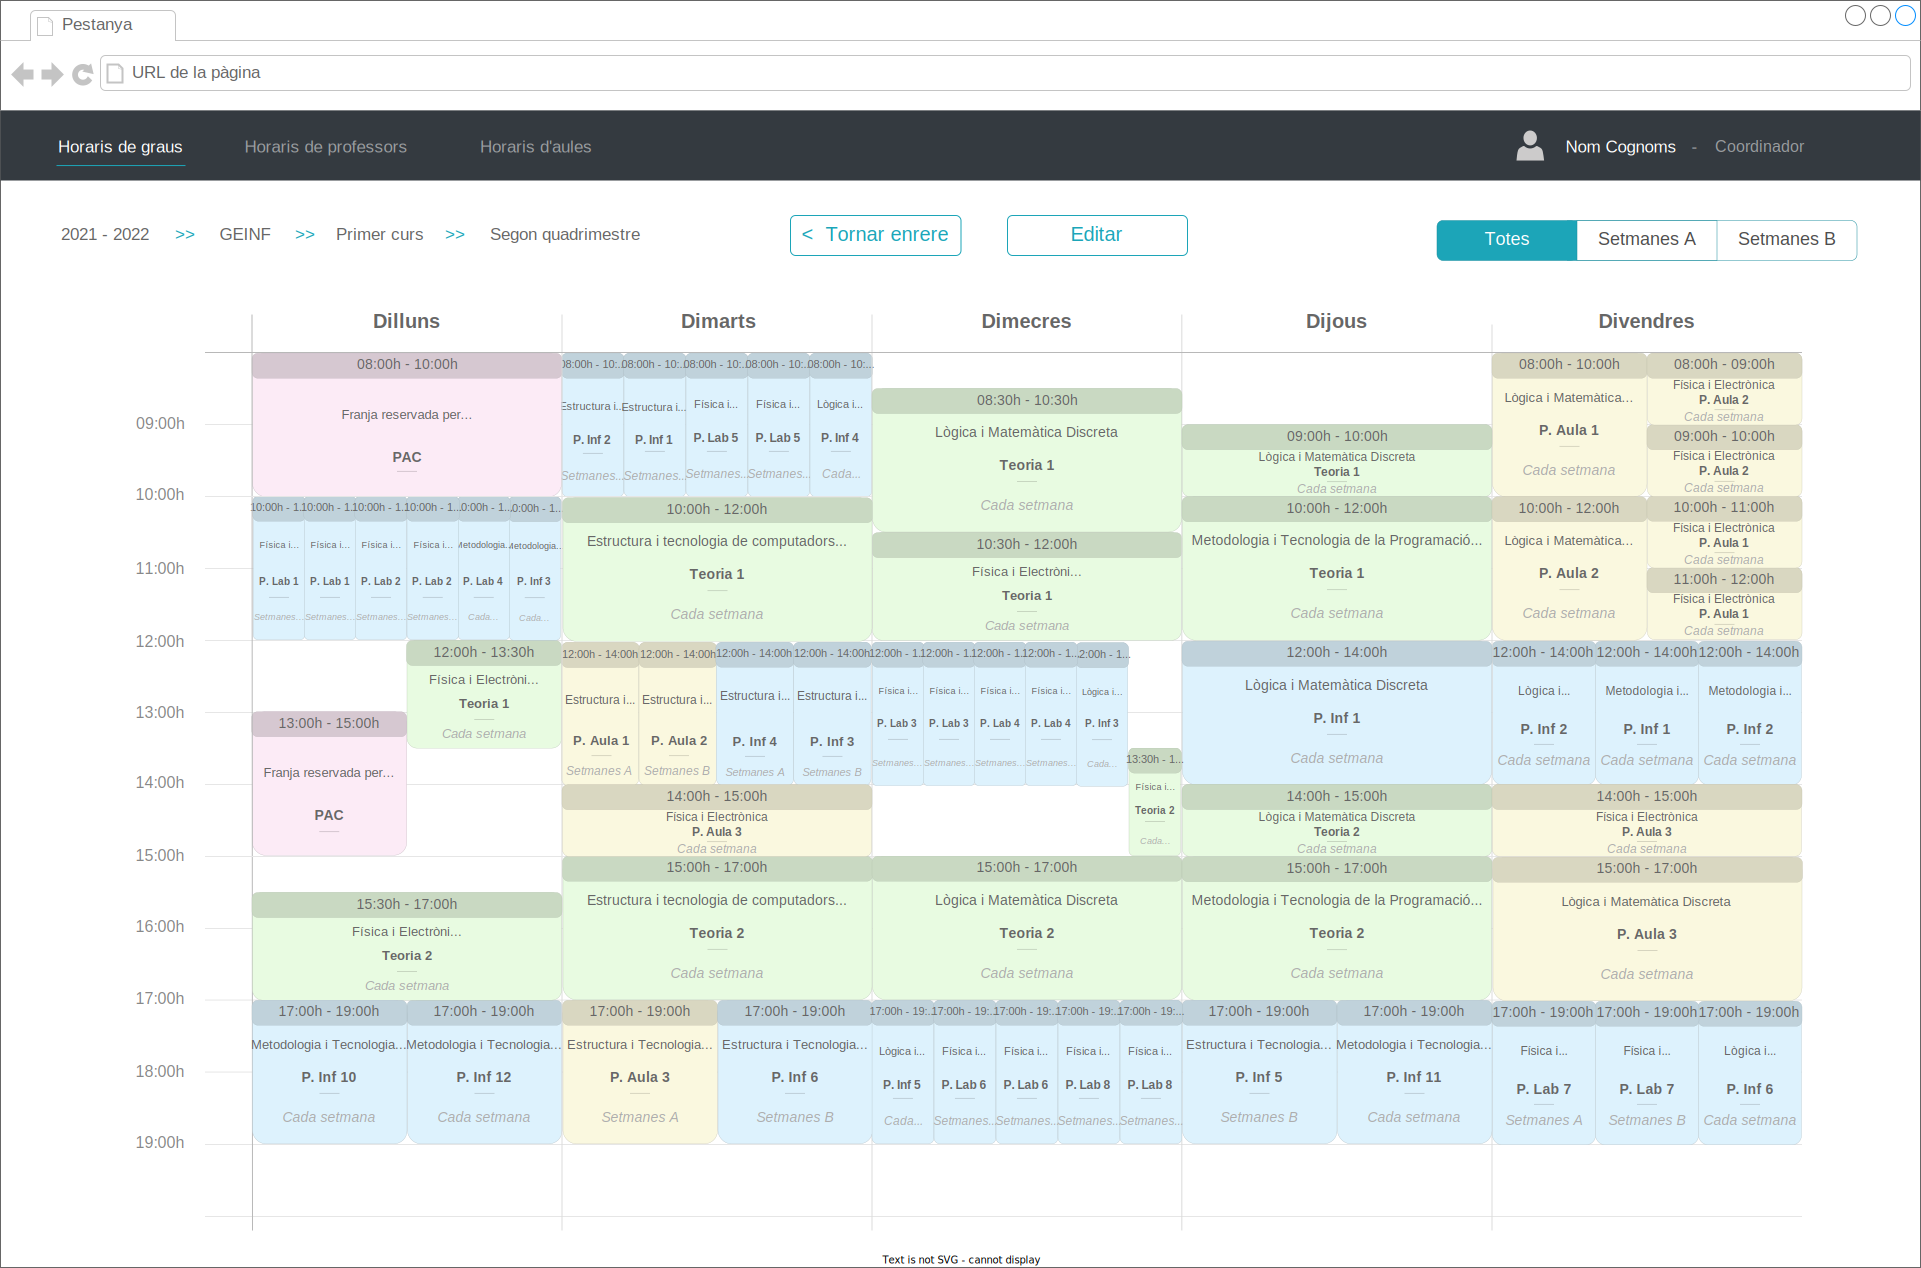
\includegraphics[width=\textwidth]{assets/interfaces/coordinadors/horarisGraus/visualitzacio.png}
	\caption{\label{img:horarisGraus_visualitzacio}Text}
\end{figure}

\begin{figure}[htpb]
	\centering
	\includegraphics[width=\textwidth]{assets/interfaces/coordinadors/horarisGraus/edicio.png}
	\caption{\label{img:horarisGraus_edicio}Text}
\end{figure}

\begin{figure}[htpb]
	\centering
	\includegraphics[width=\textwidth]{assets/interfaces/coordinadors/horarisProfessors/main.png}
	\caption{\label{img:horarisProfessors_main}Text}
\end{figure}

\begin{figure}[htpb]
	\centering
	\includegraphics[width=\textwidth]{assets/interfaces/coordinadors/horarisAules/main.png}
	\caption{\label{img:horarisAules_main}Text}
\end{figure}


\FloatBarrier
\subsection{Interfícies pels Directors de Departament}
\label{subsec:interficies_directors}

\begin{figure}[htpb]
	\centering
	\includegraphics[width=\textwidth]{assets/interfaces/directors/gestResp/main.png}
	\caption{\label{img:gestResp_main}Text}
\end{figure}

\begin{figure}[htpb]
	\centering
	\includegraphics[scale=0.3]{assets/interfaces/directors/gestResp/assignDialog.png}
	\caption{\label{img:gestResp_assignDialog}Text}
\end{figure}

\FloatBarrier
\subsection{Interfícies pels Responsables de Docècia}
\label{subsec:interficies_responsables}


\FloatBarrier
\subsection{Interfícies pels Professors}
\label{subsec:interficies_professors}



\chapter{Implementació i proves}
\label{cap:implementacio}





\chapter{Implantació i resultats}
\label{cap:implantacio}





\chapter{Conclusions}
\label{cap:conclusions}





\chapter{Treball futur}
\label{cap:treball_futur}

\begin{itemize}
  \item Poder buscar usuaris per consultar les seves dades (nom, rol, departament, telèfon, email, etc.) i habilitar un link per enviar-li un email.
  \item Que l'inicialització dels cursos no es basi en un excel, sinó que es puguin recuperar les dades de les BDD de l'escola.
  \item Sistema d'avisos i notificacions.
  \item \ldots
\end{itemize}


\backmatter

\bibliographystyle{ThesisStyleBreakable}
\bibliography{biblio}
%\printnomenclature

%\appendix

%\include{Appendix1}

\chapter*{Manual d'usuari}

\section*{Rol 1}



\section*{Rol 2}



\section*{Rol 3}



\section*{Rol 4}




\end{document}
